\documentclass[11pt]{article}

\usepackage[margin=0.6in]{geometry}
\usepackage[T1]{fontenc}
\usepackage[utf8]{inputenc}
\usepackage{lmodern}
\usepackage{array}
\usepackage{booktabs}
\usepackage{enumitem}
\usepackage{hyperref}
\usepackage{longtable}
\usepackage{parskip}
\usepackage{ragged2e}
\usepackage{setspace}
\usepackage{tabularx}
\usepackage{titlesec}
\usepackage[table]{xcolor}
\usepackage{tikz}
\usepackage[most]{tcolorbox}
\usetikzlibrary{arrows.meta,positioning,shapes.geometric,calc}

\definecolor{PrimaryRed}{HTML}{8B1E1E}
\definecolor{SoftBlue}{HTML}{DDEEFF}
\definecolor{DarkGray}{HTML}{333333}
\definecolor{SoftGreen}{HTML}{EEF6F2}
\definecolor{SoftGold}{HTML}{FFF6E6}
\definecolor{SoftPurple}{HTML}{F7F2FA}
\definecolor{SoftRose}{HTML}{FCEEEF}

\hypersetup{colorlinks=true,linkcolor=black,urlcolor=black,citecolor=black}
\setlength{\parindent}{0pt}
\setstretch{1.12}
\newcolumntype{Y}{>{\RaggedRight\arraybackslash}X}
\newcolumntype{L}[1]{>{\RaggedRight\arraybackslash}p{#1}}
\setlist[itemize]{topsep=2pt,itemsep=1pt,parsep=0pt,partopsep=0pt,leftmargin=1.2em}
\setlist[enumerate]{topsep=2pt,itemsep=2pt,parsep=0pt,partopsep=0pt,leftmargin=1.3em}
\titleformat{\section}{\large\bfseries\color{PrimaryRed}}{}{0em}{}
\titleformat{\subsection}{\normalsize\bfseries}{\thesubsection}{0.5em}{}

\newtcolorbox{ReflectionBox}{
  colback=SoftPurple,
  colframe=PrimaryRed,
  boxrule=0.8pt,
  arc=2mm,
  left=1.5mm,
  right=1.5mm,
  top=1.2mm,
  bottom=1.2mm
}

\newtcolorbox{TakeawayBox}{
  colback=SoftGreen,
  colframe=DarkGray,
  boxrule=0.6pt,
  arc=2mm,
  left=1.5mm,
  right=1.5mm,
  top=1mm,
  bottom=1mm
}

\begin{document}

\begin{titlepage}
\newgeometry{margin=0.7in}
\thispagestyle{empty}

\begin{center}
{\large University of Rochester\\}
{\normalsize Warner School of Education\\[0.15in]}

{\color{PrimaryRed}\rule{\textwidth}{1.4pt}}\\[0.12in]
{\huge\bfseries Journal Article Review\\[0.08in]
\Huge Social-Emotional Learning,\\[0.08in]
Classroom Climate, and Inclusive Design}\\[0.18in]
{\Large An Evidence-Based Reflection on the RULER Approach to SEL}\\[0.12in]
{\color{PrimaryRed}\rule{0.78\textwidth}{0.7pt}}\\[0.22in]

\colorbox{SoftBlue}{%
\parbox{0.88\textwidth}{%
\centering\small\vspace{0.02in}
\textbf{From Individual Skill-Building to Environment-Level Change}\\[0.05in]
Examining how a randomized controlled trial on the RULER SEL approach connects to inclusive, neurodiversity-affirming, and trauma-responsive classroom practice---and to my own lived experience as a Dominican immigrant navigating ADHD, chronic illness, and neurodivergence in educational systems.
% \vspace{0.02in}
}%
}
\end{center}

\vspace{0.12in}
% \vfill{}

\begin{center}
\renewcommand{\arraystretch}{1.18}
\setlength{\tabcolsep}{4pt}
\begin{tabular}{>{\bfseries\RaggedLeft}p{1.65in} p{4.9in}}
Student         & Piter Zacari Garcia Bautista \\
Course          & ED452C \\
Assignment      & Journal Article Review --- SEL / PBIS \\
Focus           & Social-emotional learning as an inclusive, environment-level intervention for neurodivergent, CLD, chronically ill, and multiply-identified students \\
Lens            & Puzzle Plan \& EQUITAS frameworks for equity-centered, neurodiversity-affirming practice \\
Submission Date & \today \\
\end{tabular}
\end{center}

\vspace{0.12in}

% -----------------------------------------------------------------------
% AUTHOR'S DISCLAIMER: Brief context for the two personal frameworks
% referenced throughout this review.
% -----------------------------------------------------------------------
\begin{center}
\begin{minipage}{0.92\textwidth}
\centering\footnotesize
\itshape
Joy-oriented literacy is not extra. It is part of access. When students feel capable, connected, and allowed to participate as themselves, literacy becomes a tool for liberation, self-determination, and empowerment.
{\color{PrimaryRed}\rule{4in}{0.5pt}}

% \vspace{0.32in}
% \vspace{0.15in}

% \vfill{}

% \upshape\tiny\RaggedRight
% \textbf{Author's Disclaimer \& Framework Context:}
% This review is written through the lens of two personal frameworks I developed to redesign exclusionary systems.
% The \textbf{Puzzle Plan} is my overarching pedagogical methodology---each lesson, activity, and intervention functions as a deliberate ``puzzle piece'' building toward intersectional, neurodivergent-inclusive, and trauma-responsive learning environments for CLD and multiply-marginalized students.
% \textbf{EQUITAS} (\textit{Equity-Quantified Unbiased Intelligence Through Algorithmic Solutions}) is the equity-centered diagnostic framework I built---originally to detect and correct bias in healthcare and educational AI---adapted here to evaluate whether classroom systems offer fair, culturally responsive, and multiple pathways for all students to access learning and demonstrate what they know.
% Both frameworks emerge directly from my lived experience as a Dominican immigrant with ADHD, chronic illness, and neurodivergent identity navigating systems not designed for people like me.
\end{minipage}
\end{center}

% \vfill{}

\begin{center}
\begin{minipage}{1.0\textwidth}
\textbf{Abstract \& Framework Context}\\[-0.03in]
% \small
This journal article review examines Rivers, Brackett, Reyes, Elbertson, and Salovey (2013), an empirical clustered randomized controlled trial published in \textit{Prevention Science} that tested the RULER Approach to social-emotional learning (SEL) in upper-elementary classrooms across a large urban district. The study found that RULER classrooms showed significantly warmer teacher--student relationships, greater student autonomy, and stronger teacher responsiveness to student interests compared to control classrooms. This review summarizes the study's methods, findings, and implications while reflecting on what the evidence means for inclusive classrooms serving neurodivergent, culturally and linguistically diverse (CLD), chronically ill, trauma-experienced, and multiply identified students. I read these findings through my Puzzle Plan and EQUITAS frameworks, which emerge from my lived experience as a Dominican immigrant with ADHD, chronic illness, and neurodivergent identity. From that lens, RULER matters because it shows that SEL is not a soft add-on or isolated skill lesson; it is an environment-level intervention that can reshape classroom climate, belonging, equity, and access.
\end{minipage}
\end{center}

\restoregeometry
\end{titlepage}
\clearpage

{\LARGE\bfseries\color{PrimaryRed} Journal Article Review and Reflection\par}

\begin{center}
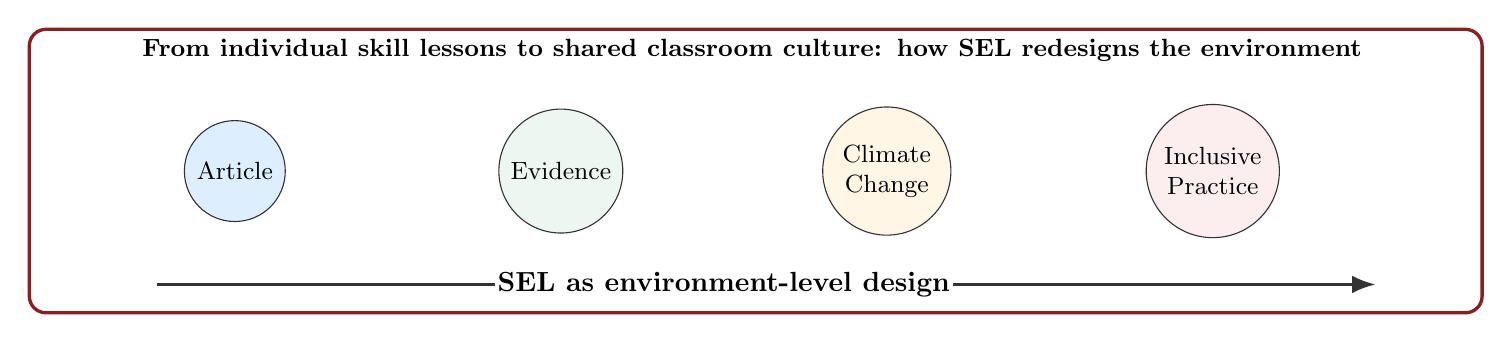
\begin{tikzpicture}[scale=1.8, every node/.style={font=\small, align=center}]
  \draw[rounded corners=6pt, very thick, PrimaryRed] (-5.9,-0.5) rectangle (4.35,1.5);
  \node[font=\small\bfseries, align=center, text width=18.0cm] at (-0.8,1.35)
  {From individual skill lessons to shared classroom culture: how SEL redesigns the environment};
  \node[circle, fill=SoftBlue,  draw=DarkGray, minimum size=1.20cm] at (-4.45,0.5) {Article};
  \node[circle, fill=SoftGreen, draw=DarkGray, minimum size=1.20cm] at (-2.15,0.5) {Evidence};
  \node[circle, fill=SoftGold,  draw=DarkGray, minimum size=1.00cm] at (0.15,0.5) {Climate \\ Change};
  \node[circle, fill=SoftRose,  draw=DarkGray, minimum size=1.30cm] at (2.45,0.5) {Inclusive \\ Practice};
  \draw[very thick, -{Latex[length=3mm]}, DarkGray] (-5.0,-0.3) -- (3.6,-0.3);
  \node[font=\bfseries, fill=white, inner sep=1pt] at (-1.0,-0.3) {SEL as environment-level design};
\end{tikzpicture}
\end{center}

\begin{ReflectionBox}
\textbf{Guiding claim.} A social-emotional learning program does not merely teach students to manage feelings. When implemented at the classroom level, it changes the relational and emotional environment so that students with neurodivergent profiles, chronic illness, trauma histories, and multiple marginalized identities can access learning without having to first perform neurotypicality or emotional control as the price of belonging. This is precisely the gap my Puzzle Plan is designed to close---and the standard my EQUITAS framework holds every classroom system accountable to.
\end{ReflectionBox}

\section{Article and APA Citation}

Rivers, S. E., Brackett, M. A., Reyes, M. R., Elbertson, N. A., \& Salovey, P. (2013). Improving the social and emotional climate of classrooms: A clustered randomized controlled trial testing the RULER Approach. \textit{Prevention Science, 14}(1), 77--87. \url{https://doi.org/10.1007/s11121-012-0305-2}

\section{Summary of Key Information}

This empirical study examined whether the RULER Approach to SEL could improve the observed social and emotional climate of upper-elementary classrooms in a large urban district. The RULER Approach was developed at the Yale Center for Emotional Intelligence and provides teachers with tools, language, and instructional routines for integrating emotional recognition, understanding, labeling, expression, and regulation into daily academic instruction. The program is designed to be embedded into existing content rather than delivered as a stand-alone curriculum period---an approach that mirrors how I designed the Puzzle Plan: not as an intervention extracted from real life, but as the architecture of everyday learning.

\subsection{Design and Sample}

The study used a clustered randomized controlled trial, which is one of the strongest experimental designs available for educational research. Sixty-two schools were randomly assigned to either implement RULER in their fifth- and sixth-grade English language arts classrooms or to continue their standard practice as a comparison condition. Because students are nested within classrooms and classrooms are nested within schools, the authors used hierarchical linear modeling to account for that nesting structure and produce valid estimates of RULER's effect.

\subsection{Measures and Findings}

Trained and independent observers rated classroom climate using a structured observation tool with subscales for teacher--student warmth, student--student connection, student autonomy and leadership, and teacher responsiveness to student interests. Observers did not know which condition a classroom was assigned to, which reduces observer bias.

Compared to control classrooms, RULER classrooms scored significantly higher on teacher--student warmth and connectedness, student opportunities for autonomy and leadership, and teacher focus on student motivation and interest rather than only task completion. These differences were not explained by pre-existing school-level differences because randomization controlled for selection bias. The findings suggest that the RULER Approach produced real, observable changes in how teachers and students related to each other during ordinary academic time.

\subsection{Interpretation and Significance}

The authors argue that classroom climate is a key mechanism through which SEL programs promote positive youth development. A climate that is warmer, more autonomy-supportive, and more responsive to student interests creates the conditions for students to engage, take risks, and ask for help. Importantly, the study measured climate through observation rather than self-report, which strengthens confidence that the changes reflect actual instructional behavior rather than just teachers' beliefs about themselves.

\begin{TakeawayBox}
\textbf{Study snapshot.} Sixty-two urban schools, randomized design, trained observers, multi-level modeling. RULER classrooms showed measurably warmer relationships, greater student autonomy, and stronger teacher responsiveness --- effects large enough to be detected through structured observation across an entire school year.
\end{TakeawayBox}

\section{What I Learned and Why It Matters}

\begin{ReflectionBox}
\textbf{Learning and reflection.} This article shifted my understanding of SEL from a lesson-delivery model to a climate-design model---and that reframing maps directly onto the Puzzle Plan's core principle: environment is the intervention. RULER did not just teach students about emotions; it changed what the classroom felt and functioned like. That is what the Puzzle Plan attempts in every lesson design decision I make, and it is what EQUITAS holds diagnostic and instructional systems accountable for: not just whether a tool is technically accurate, but whether it creates conditions where marginalized students are seen, heard, and positioned as capable.
\end{ReflectionBox}

\subsection{SEL as Access, Not Just Wellness}

The most important thing I learned from this article is that a consistently warm, autonomy-supportive, and emotionally literate classroom is not a nice-to-have feature. For students with ADHD, depression, anxiety, autism, chronic illness, trauma histories, or complex intersecting identities, the emotional quality of the environment determines whether learning is even possible. I know this from the inside. My own years of academic struggle---where ADHD and an undiagnosed chronic illness created a vicious cycle of poor performance, shame, depressive episodes, and avoidance---were not failures of motivation. They were failures of environment. Rigid assessment formats with no backtracking, unclear structure, and no flexibility for how my brain works transformed competence into collapse. RULER's changes to teacher warmth and responsiveness are, from that perspective, a form of Universal Design for Learning: they reduce the cognitive and emotional load that students with disabilities carry into every lesson. EQUITAS asks exactly this question about every tool and task: does it create multiple, fair pathways, or does it demand that students perform normalcy as the price of access?

\subsection{Climate as a Bridge Between SEL and Disability Supports}

This study also helped me see that SEL and disability support do not have to operate in separate tracks. When a teacher uses emotion language daily, co-creates classroom norms, and responds to student interests as a routine practice, the result is a classroom where a student can say ``I am overwhelmed'' or ``I need a break'' without being marked as the student with the IEP. That normalization matters because neurodivergent and disabled students often report that the stigma of being singled out for support is itself a barrier to using those supports---a dynamic I experienced directly, where being identified as different compounded the distress of already struggling. RULER's infusion model---integrating SEL into English language arts rather than treating it as a weekly feelings lesson---is a powerful model for how Puzzle Plan design principles work: every lesson is an opportunity to build the relational infrastructure that makes differentiation invisible, not stigmatizing.

\subsection{Implementation Quality and Equity}

The article also pushed me to think carefully about implementation through an EQUITAS lens. Even a well-designed, evidence-based program can be reduced to surface compliance if teachers use the emotion vocabulary only as a classroom management tool or if the program is delivered inconsistently across CLD student populations. For example, a student who is a recent English language learner, a student whose family communicates distress differently from the dominant culture, or a student experiencing housing instability may need more than warmth and autonomy in the classroom. As I encountered with my own chronic illness---dismissed as psychological by a specialist who had already decided I was fabricating symptoms---being in a warmer environment does not always undo the damage of being disbelieved by systems for years. SEL has to be paired with structural responsiveness, culturally sustaining relationship-building, and material support. The Puzzle Plan builds in this layer explicitly: each piece of the environment must be interrogated through the intersectional lens of who it serves and who it invisibilizes.

\subsection{Connection to Transition and Adult Readiness}

Finally, the study connects to our course's transition planning thread. Students with disabilities who spend their K--12 years in classrooms where help-seeking is normalized, where autonomy is practiced, and where emotional literacy is a shared language are better positioned to self-advocate in college, workplace, and community settings. I think about the years I spent not knowing I could name what was happening in my body and brain---and how much that silence cost me academically, medically, and emotionally. Transition planning focuses on skills and services, but it often underestimates the role of the relational environment in building the confidence to use those skills. A student who has experienced years of co-regulation, warm correction, and responsive adult relationships is more likely to ask for accommodations at a disability services office or disclose a health need to an employer than a student whose school experience was characterized by surveillance and compliance management.

\begin{ReflectionBox}
The RULER study gave me language for something I have been trying to articulate across every course in this program, in my Puzzle Plan work, and in the EQUITAS framework: the difference between a school that accommodates disability and a school that designs for it. Accommodation is reactive; design is proactive. SEL, when implemented at the classroom climate level, is one of the most scalable, evidence-backed tools we have for proactive, environment-level inclusive design---and for making sure that students who look like me, and live like I did, do not have to wait years to be believed.
\end{ReflectionBox}

\newpage
\section*{References}
\small
Brackett, M. A., Rivers, S. E., Reyes, M. R., \& Salovey, P. (2012). Enhancing academic performance and social and emotional competence with the RULER feeling words curriculum. \textit{Learning and Individual Differences, 22}(2), 218--224. \url{https://doi.org/10.1016/j.lindif.2010.10.002}

CASEL. (n.d.). \textit{What is the CASEL framework?} \url{https://casel.org/fundamentals-of-sel/what-is-the-casel-framework/}

ED452C. (n.d.). \textit{Journal Article Review Directions and Rubric}. Course handout.

Garcia Bautista, P. Z. (2025). \textit{EQUITAS: Equity-Quantified Unbiased Intelligence Through Algorithmic Solutions --- A framework for fairness-aware diagnostics in CLD populations}. Unpublished framework, Rochester Institute of Technology.

Individuals with Disabilities Education Act, 34 C.F.R.\ \S\S\ 300.43, 300.320, 300.321. \url{https://sites.ed.gov/idea/regs/}

Rivers, S. E., Brackett, M. A., Reyes, M. R., Elbertson, N. A., \& Salovey, P. (2013). Improving the social and emotional climate of classrooms: A clustered randomized controlled trial testing the RULER Approach. \textit{Prevention Science, 14}(1), 77--87. \url{https://doi.org/10.1007/s11121-012-0305-2}

Ter-Minassian, H., Wong, J., Lekadir, K., \& Baams, L. (2022--2025). \textit{Fairness-aware machine learning for CLD adolescent diagnostic equity: A cross-study synthesis}. [Multiple peer-reviewed sources synthesized across ED415 and IDAI700 research portfolio]. Rochester Institute of Technology.

\end{document}efg